\documentclass{article}
\usepackage{titling}
\usepackage{parskip}
\usepackage{setspace}
\usepackage[utf8]{inputenc}
\usepackage{amsmath, amsthm, amssymb, amsfonts, mathtools, xfrac, dsfont}
\usepackage[labelfont=bf]{caption}
\usepackage[labelfont=bf]{subcaption}
\usepackage{float}
\usepackage[margin=0.8in]{geometry}
\usepackage{algorithm}
\usepackage{algorithmic}
\usepackage{xcolor}
\usepackage[export]{adjustbox}
\usepackage{hyperref}
\usepackage{tabularx}
\usepackage{makecell}
\usepackage{bm}
\usepackage{indentfirst}

\newcommand{\norm}[1]{\left\lVert#1\right\rVert}
\newcommand{\abs}[1]{\left|#1\right|}
\newcommand{\mat}[1]{\begin{bmatrix}#1\end{bmatrix}}
\renewcommand{\arraystretch}{1.3}
\newcommand{\R}{\mathbb{R}}
\newcommand{\Z}{\mathbb{Z}}
\newcommand{\E}{\mathbb{E}}
\newcommand{\N}{\mathcal{N}}
\newcommand{\I}{\mathcal{I}}
\renewcommand{\S}{\mathbb{S}}
\DeclareMathOperator{\tr}{tr}
\DeclareMathOperator{\Cov}{Cov}
\DeclareMathOperator{\diag}{diag}
\DeclarePairedDelimiter\floor{\lfloor}{\rfloor}
\DeclarePairedDelimiter\ceil{\lceil}{\rceil}
\DeclareMathOperator*{\argmax}{arg\,max}
\DeclareMathOperator*{\argmin}{arg\,min}

\captionsetup{justification=centering}
\numberwithin{equation}{section}
\setlength\parindent{0.25in}
\setstretch{1.1}

% covariance matrix
\newcommand{\cm}{\bm{\Sigma}}
% approximate covariance matrix
\newcommand{\acm}{\widetilde{\cm}}
\newcommand{\x}{\bm{x}}
\newcommand{\xp}{\bm{x'}}
\newcommand{\y}{\bm{y}}
\newcommand{\a}{\bm{a}}
\renewcommand{\c}{\bm{c}}
\renewcommand{\u}{\bm{u}}
\newcommand{\v}{\bm{v}}
\newcommand{\A}{\bm{A}}
\newcommand{\U}{\bm{U}}
\newcommand{\V}{\bm{V}}
\newcommand{\W}{\bm{W}}

\title{\textbf{Scalable Global Parameter Estimation for Nonstationary Gaussian Processes}}
\date{}
\author{
Paul G. Beckman\thanks{Mathematics and Computer Science Division, Argonne National Laboratory} \and
Christopher J. Geoga\footnotemark[1] \thanks{Department of Statistics, Rutgers University} \and
Mihai Anitescu\footnotemark[1] \thanks{Department of Statistics, University of Chicago}
}

\begin{document}

\maketitle

\vspace{-2\baselineskip}

\begin{abstract}
Put the abstract here.
\end{abstract}

\section{Introduction}

Gaussian process assumptions and applications overview.

\begin{equation}
  -\ell(\bm{\theta}) := \frac{1}{2}\log\abs{\cm(\bm{\theta})} + \frac{1}{2}(\y-\bm{\mu})^\top\cm(\bm{\theta})^{-1}(\y-\bm{\mu}) + \frac{n}{2}\log(2\pi)
  \label{eqn:nll}
\end{equation}

Minimizing \ref{eqn:nll} numerically can be computationally expensive, as conventional determinant and linear solve operations scale cubically in time and quadratically in storage. As $n$ grows, the evaluation of \ref{eqn:nll} thus becomes prohibitively expensive. In response to these scaling challenges, a number of methods have been introduced to more efficiently compute or approximate \ref{eqn:nll}.

Fast Gaussian process MLE methods (Vecchia, Guinness, Chen-Stein, Anitescu-Stein, Lindgren, Minden, Geoga, Ambikasaran). We choose to use HODLR, see Section \ref{sec:hodlr}.

With the exception of \cite{guinness2019gaussian}, all of these scalable methods are applied exclusively to stationary models. However, stationarity is often an unrealistic assumption for large datasets spanning spatial regions in which small scale dynamics cause variation in the local behavior of the data. To address this issue, past work has used locally stationary models in which the parameters of the random field are assumed to be constant in some neighborhood. Both disjoint neighborhoods \cite{lenzi2019improving} and overlapping or moving window neighborhoods \cite{kuusela2018locally, anderes2011local} have been used for maximum likelihood parameter estimation and prediction. Under such approaches, one must perform parameter estimation and prediction using only the observations lying in a single neighborhood instead of using the entire set of observations, as the stationary GP model is only assumed locally. Thus one must choose the neighborhood size a priori to balance the spatial scale of the nonstationary with the density of observations such that the neighborhoods are small enough to capture local variation but contain sufficient observations to make accurate predictions. The scalability of matrix operations using the HODLR-approximated covariance $\bm{\widetilde{\Sigma}}$ allows us to use the full dataset for parameter estimation and prediction, sidestepping the question of neighborhood size.

Apart from locally stationary models, significant effort has been devoted to the construction of positive definite nonstationary covariance functions with spatially varying parameters \cite{gibbs1997bayesian, paciorek2003nonstationary}. Stein \cite{stein2005nonstationary} introduces the following Mat\'ern covariance function with spatially varying anisotropy $\Lambda : \Omega \to \mathbb{S}^d_{++}$, variance $\sigma^2 : \Omega \to \R_+$, and smoothness $\nu : \Omega \to \R_+$
\begin{equation}
  k(\x, \xp) := \sigma^2(\x) \sigma^2(\xp) \abs{\frac{\Lambda(\x) + \Lambda(\xp)}{2}}^{-\frac{1}{2}}
  \mathcal{M}_{\frac{\nu(\x) + \nu(\xp)}{2}} \bigg( \sqrt{Q_{ij}} \bigg)
  \label{eqn:covfunc}
\end{equation}
using the quadratic form
\begin{equation*}
  Q_{ij} := (\x - \xp)^\top \Big(\frac{\Lambda(\x) + \Lambda(\xp)}{2}\Big)^{-1} (\x - \xp),
\end{equation*}
where $\mathcal{M}_\nu$ is the stationary isotropic Mat\'ern covariance function
$$ \mathcal{M}_\nu(r) := \frac{2^{1-\nu}}{\Gamma(\nu)} (\sqrt{2\nu} r)^\nu K_\nu(\sqrt{2\nu} r) $$
and $K_\nu$ is the modified Bessel function of the second kind of order $\nu$.

In order to compute the nonstationary covariance function \ref{eqn:covfunc}, one must specify the spatially varying parameter functions $\Lambda, \sigma^2,$ and $\nu$. Asymptotic results show that the parameters $\sigma^2$ and $\Lambda$ cannot be consistently estimated simultaneously using an increasing number of observations in a bounded subset of $\R^p$ for $p<4$, even when they are not spatially varying and $\Lambda = \lambda I$ is restricted to be a scalar multiple of the identity \cite{zhang2004inconsistent}.
Thus for identifiability purposes the spatially varying parameter functions $\Lambda, \sigma^2,$ and $\nu$ must be severely restricted. For the purpose of concreteness and demonstration within this manuscript, we will assume $\nu$ is fixed and known, estimating either $\Lambda$ or $\sigma^2$ and fixing the other.

Many authors have adopted a Bayesian approach to estimating a spatially varying parameter function $\theta \in \{\Lambda, \sigma^2\}$ by specifying a prior over some functional space and sampling the posterior distribution using Markov Chain Monte Carlo \cite{risser2015regression, gibbs1997bayesian, paciorek2004nonstationary, paciorek2006spatial, higdon1998process}. Alternatively, within the maximum likelihood framework the covariance matrix $\cm[\theta]$ becomes a functional which depends on the parameter function $\theta$. Minimizing the negative log likelihood \ref{eqn:nll} thus becomes a variational problem, which we solve approximately by estimating $\theta$ as a linear combination of basis functions $\{ \psi_i\}_{i=1}^m$,
\begin{equation}
  \min_{\theta : \Omega \to D} -\ell[\theta] \approx \min_{\a \in \R^m} -\ell\Bigg[\sum_{i=1}^m a_i \psi_i\Bigg],
  \label{eqn:var}
\end{equation}
where $D$ is the domain on which $\theta$ is a valid parameter. Our choices of parameterization and basis set determine the structure of the resulting optimization problem. For example, in the case of estimating a positive parameter like $\sigma^2$ using a set of positive basis functions, we obtain the bound constrained nonlinear program
\begin{equation}
  \begin{aligned}
    \min_{\a \in \R^m} & -\ell\Bigg[ \sum_{i=1}^m a_i \psi_i \Bigg] \\
    a_i & \geq 0 \quad \forall \ i=1,...,m.
    \label{eqn:opt}
  \end{aligned}
\end{equation}
We use radial basis functions (RBFs), for example the Gaussian functions $\psi_i(\x) = e^{-\frac{\norm{\x - \c_i}^2}{r}}$, centered at $\c_i$ so that the estimated function $\sigma^2$ is everywhere positive, and we normalize these functions so that $\sum_{i=1}^m \psi_i(\x) = 1$. The principle advantage of normalization is that for small values of the radius parameter $r$, linear combinations of the basis functions approach piecewise constant functions, which is a more meaningful estimator than the sum of delta functions approached in the same small $r$ limit without normalization. In addition, the RBF sets yield localized dependence, allowing additional approximations which reduce computational cost, see Section \ref{sec:computation}. However, we emphasize that the above framework is applicable to any basis set, for example polynomial or Fourier bases, if one chooses to estimate a transformed variable, such as $\log(\sigma^2)$ which is not required to be positive.

% \begin{figure}[t!]
%   \centering
%   \begin{subfigure}[t]{0.2\textwidth}
%     \includegraphics[width=\textwidth]{figures/rbfs.pdf}
%     \caption{}
%   \end{subfigure}%
%   \begin{subfigure}[t]{0.2\textwidth}
%     \includegraphics[width=\textwidth]{figures/nrbfs.pdf}
%     \caption{}
%   \end{subfigure}
%   \caption{Unnormalized (a) and normalized (b) Gaussian basis sets on [0,1] with centers at 0.2, 0.4, 0.6, and 0.8.}
%   \label{fig:rbf}
% \end{figure}

\section{HODLR matrices and scalable likelihood computations} \label{sec:hodlr}
We now provide a brief overview of HODLR matrices and methods for computing the likelihood and its gradient and hessian in quasilinear time. A symmetric HODLR matrix is of the form
\begin{equation}
  \mat{\A_1 & \U \V^\top \\ \V \U^\top & \A_2}
  \label{eqn:hodlr}
\end{equation}
where $\U, \V \in \R^{n \times p}$ and $\A_1$ and $\A_2$ are either dense or of the form \ref{eqn:hodlr}.

\begin{equation}
  \big[-\nabla \ell(\bm{\theta}) \big]_j = \frac{1}{2} \tr(\cm^{-1} \cm_j) - \frac{1}{2} \y^\top \acm^{-1} \acm_j \acm^{-1} \y
  \label{eqn:grad}
\end{equation}

\begin{equation}
  \tr(\acm^{-1} \acm_j) \approx \frac{1}{2N_h} \sum_{i=1}^{N_h} \u_i^\top \acm^{-1} \acm_j \u_i
  \label{eqn:hutch}
\end{equation}

\begin{equation}
  \frac{1}{2N_h} \sum_{i=1}^{N_h} \u_i^\top \W^{-1} \acm_j \W^{-\top} \u_i
  \label{eqn:symhutch}
\end{equation}

\begin{equation}
  \big[-\nabla \tilde{\ell}(\bm{\theta}) \big]_j \approx \frac{1}{2N_h} \sum_{i=1}^{N_h} \u_i^\top \W^{-1} \acm_j \W^{-\top} \u_i - \frac{1}{2} \y^\top \acm^{-1} \acm_j \acm^{-1} \y
  \label{eqn:approxgrad}
\end{equation}

\begin{equation}
  \I_{jk} = \frac{1}{2} \tr(\acm^{-1} \acm_j \acm^{-1} \acm_k)
  \label{eqn:fish}
\end{equation}

\begin{equation}
  \widehat{\I}_{jj} = \frac{1}{2N_h} \sum_{i=1}^{N_h} \u_i^\top \W^{-1} \acm_j \acm^{-1} \acm_j \W^{-\top} \u_i
  \label{eqn:approxfishdiag}
\end{equation}

\begin{equation}
  \widehat{\I}_{jk} = \frac{1}{4N_h} \sum_{i=1}^{N_h} \u_i^\top \W^{-1} (\acm_j + \acm_k) \acm^{-1} (\acm_j + \acm_k) \W^{-\top} \u_i - \frac{1}{2} \widehat{\I}_{jj} - \frac{1}{2} \widehat{\I}_{kk}
  \label{eqn:approxfish}
\end{equation}

\begin{equation}
  \big[-\nabla^2 \tilde{\ell}(\bm{\theta})\big]_{jk} = -\I_{jk} + \frac{1}{2} \tr(\acm^{-1} \acm_{jk}) - \frac{1}{2} \y^\top \Big( \frac{\partial}{\partial \theta_k} \acm^{-1} \acm_j \acm^{-1} \Big) \y
  \label{eqn:approxhess}
\end{equation}

\begin{equation}
  \frac{\partial}{\partial \theta_k} \acm^{-1} \acm_j \acm^{-1} = - \acm^{-1} \acm_k \acm^{-1} \acm_j \acm^{-1} + \acm^{-1} \acm_{jk} \acm^{-1} - \acm^{-1} \acm_k \acm^{-1} \acm_j \acm^{-1}
  \label{eqn:derexp}
\end{equation}


\section{Computational considerations} \label{sec:computation}
Although the HODLR approximation greatly improves the scalability of the evaluation of the likelihood and its derivatives, the nonlinear programs resulting from the basis function formulation \ref{eqn:var} become high-dimensional and costly when a large number of basis functions are used. The computational expense of these problems stems both from the cost of evaluating the covariance function and from the number of entries in the gradient and hessian. Computing the local parameter as a linear combination of basis function values scales as $O(m)$, dominating the other $O(1)$ arithmetic operations in evaluating the covariance function \ref{eqn:covfunc}. In addition, the nonlinear program has $m$ variables, resulting in $m$ gradient entries and $m^2$ hessian entries. Thus evaluating the likelihood scales as $O(m n\log n)$, the gradient as $O(m^2 n\log n)$, and the hessian as $O(m^3 n\log n)$. In order to capture fine-scale variation in the parameter function, one must often use a relatively large basis set, for which this scaling is not computationally feasible. We now discuss methods which improve the computational complexity of identifying local minima in these nonlinear programs.

\subsection{Scalable quasi-Newton algorithms}
Full Newton-Raphson and Fisher scoring overview

By using a radial basis set, the effect of the variable $a_i$ on the linear combination is concentrated near the RBF center $c_i$. Combined with the monotonic decay of the Mat\'ern covariance function as $\norm{\x - \xp}$ grows, we expect that $\frac{\partial^2}{\partial a_i \partial a_j}$ will be small when the RBF centers $\c_i$ and $\c_j$ are far apart. Experimentally, we see that for sufficiently localized RBFs, the hessian displays rapid off-diagonal decay, see Figure \ref{fig:hess}. This concentration of second order information on the diagonal of the Hessian indicates that an approximation by a hierarchical or diagonal matrix may facilitate scalable quasi-Newton methods. So-called quasi-Cauchy methods \cite{zhu1999quasi, andrei2019diagonal} have been previously proposed, computing sequential updates to a diagonal Hessian approximation satisfying a weak secant equation \cite{dennis1993sizing}. We propose a simpler approach in which we extract the diagonal elements of the Fisher or Hessian matrix and use this diagonal matrix directly as an approximation to the full matrix.

% \begin{figure}[t!]
%   \centering
%   \begin{subfigure}[t]{0.3\textwidth}
%     \includegraphics[width=\textwidth]{figures/hessians/p1000-a20.pdf}
%     \caption{Hessian}
%   \end{subfigure}%
%   \begin{subfigure}[t]{0.3\textwidth}
%     \includegraphics[width=\textwidth]{figures/hessians/p1000-a20-log.pdf}
%     \caption{Log absolute value of Hessian}
%   \end{subfigure}
%   \caption{Hessian for the variable scale problem.}
%   \label{fig:hess}
% \end{figure}

\begin{figure}[t!]
  \begin{subfigure}[t]{0.5\textwidth}
    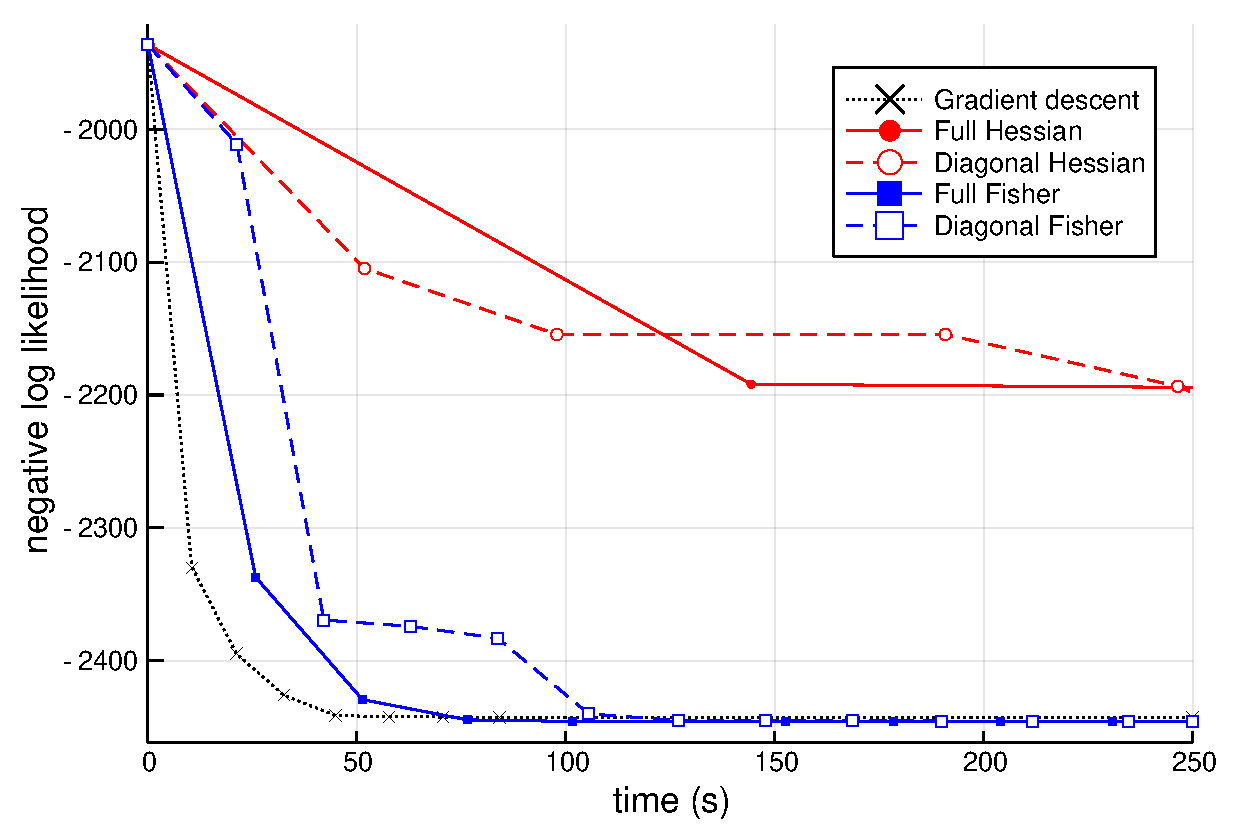
\includegraphics[width=\textwidth]{figures/timing/p1000-a20-plot.pdf}
    \caption{1000 observations with 20 anchors}
  \end{subfigure}%
  \begin{subfigure}[t]{0.5\textwidth}
    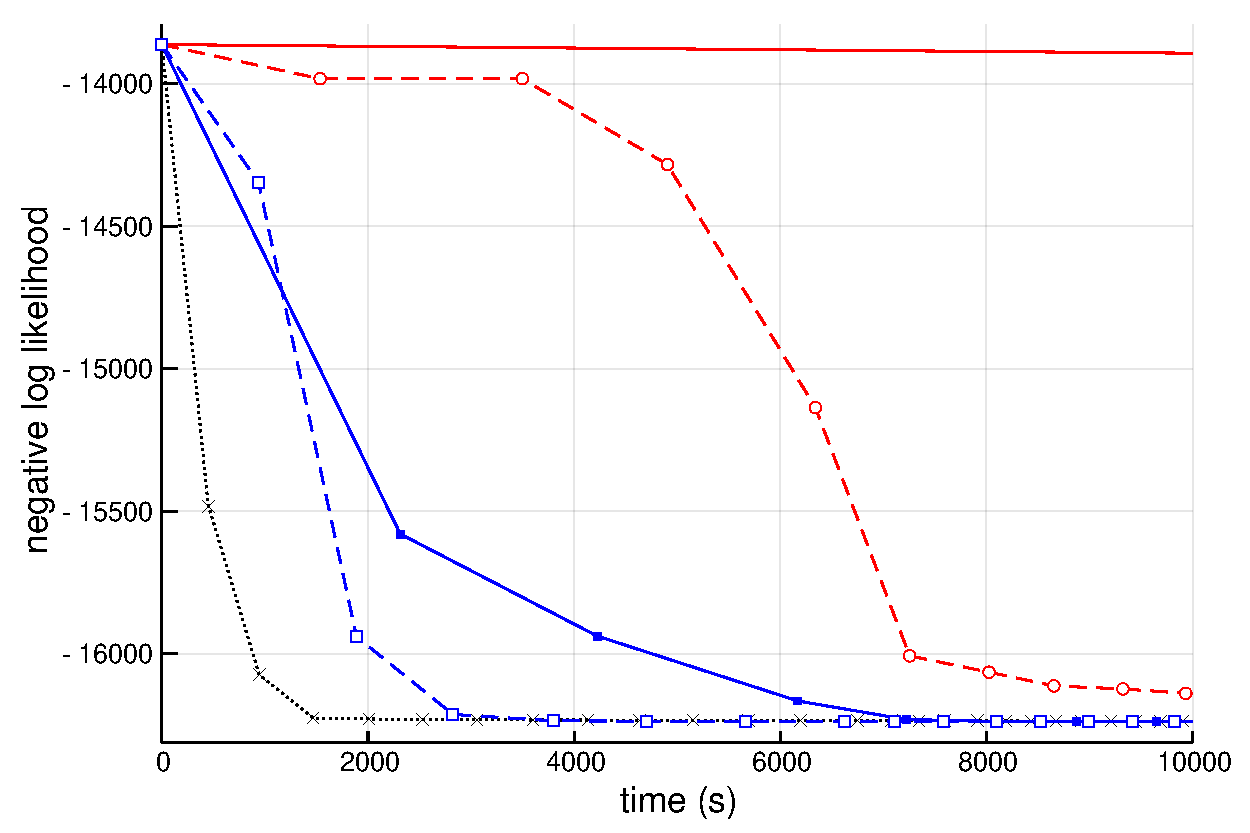
\includegraphics[width=\textwidth]{figures/timing/p5000-a50-plot.pdf}
    \caption{5000 observations with 50 anchors}
  \end{subfigure}
  \caption{Runtime comparison of gradient descent, Newton's method using the full Hessian and its diagonal, as well as Fisher scoring using the full Fisher-information matrix and its diagonal.}
  \label{fig:timing}
\end{figure}

\subsection{Compactly supported radial basis functions}

We can reduce the computational complexity of both the covariance function evaluation and the computation of the gradient and Hessian by using a compactly supported radial basis set in place of the Gaussians. We use the radial functions $\phi_{\ell,k}$ introduced by Wendland \cite{wendland1995piecewise}, defined by
\begin{equation}
  \phi_{\ell,k}(t) & = \begin{cases}
    \displaystyle\frac{1}{\Gamma(k)2^{k-1}} \int_t^1 s(1-s)^\ell(s^2-t^2)^{k-1} ds & \text{for} \ 0 \leq t \leq 1 \\
    0 & \text{for} \ t > 1
\end{cases}
\end{equation}
By setting $\ell = \floor{d/2}+k+1$ and defining $\psi_i(\x}) = \phi_{\ell,k}(\norm{\x - \c_i}/r)$, we obtain the unique piecewise polynomial radial function $\psi_i \in \mathcal{C}^{2k}(\R^d)$ of minimal degree which is zero outside of the disk of radius $r$ centered at $\c_i$. These functions have convenient recursive definitions which give simple polynomial expressions for a given smoothness $2k$ and spatial dimension $d$ \cite{fasshauer1998smoothing}. For example, $\phi_{3,1}(t) = (1-t)^4_+(4t+1)$ gives radial functions $\psi_i \in \mathcal{C}^2(\R^2)$.

Although Gaussian RBFs truncated at radius $r$ would yield a similar compactly supported basis set, this would introduce a discontinuity in the estimated parameter function on the boundary of their support at $\norm{\x - \c_i} = r$. We choose to employ the Wendland functions because we can enforce an arbitrary level of smoothness at the boundary of their support. A Gaussian process is $k$-times mean square differentiable if and only if its covariance function is $2k$ times differentiable at the origin \cite{stein1999interpolation}. Thus we can maintain the $\floor{\nu}$-times mean-squared differentiability of the Mat\'ern process with smoothness parameter $\nu$ by using the appropriate $2\floor{\nu}$ times differentiable Wendland basis functions.
% With an appropriate scaling of the radius parameter $r$, the Wendland radial basis functions approach Gaussians as the smoothness level $k \to \infty$ \cite{chernih2014wendland} and can thus be viewed as a smooth compactly supported approximation to the Gaussian basis set as opposed to the discontinuous Gaussian-like set generated by truncation.
It is also worth emphasizing that the use of a compactly supported basis functions to approximate a nonstationary parameter function does not result in a compactly supported covariance function as described by Gneiting \cite{gneiting2002compactly} or induced by covariance tapering \cite{furrer2006covariance, kaufman2008covariance}. The Mat\'ern covariance function \ref{eqn:covfunc} remains globally supported irrespective of its parameter values and the basis used to construct them.

The first advantage of compactly-supported basis functions is to reduce the cost of kernel evaluation from $O(m)$ to $O(a)$ where $a$ is the maximum number of basis functions which are simultaneously nonzero, as the linear combination contains at most this many terms. Furthermore, sparsity in $\acm_j$ and $\acm_{jk}$ induced by compactly-supported radial basis functions can improve the computational complexity of gradient and Hessian calculations. Let $S_j$ be the compact support of basis function $j$. Then applying the chain rule, writing $\theta = \theta(\bm{x})$ and $\theta' = \theta(\bm{x'})$ for convenience, we have
\begin{align*}
  \frac{\partial k(\bm{x}, \bm{x'})}{\partial a_j}
  % & = \frac{\partial \theta}{\partial a_j} \frac{\partial k(\bm{x}, \bm{x'})}{\partial \theta} + \frac{\partial \theta'}{\partial a_j} \frac{\partial k(\bm{x}, \bm{x'})}{\partial \theta'} \\
  & = \psi_j(\bm{x}) \frac{\partial k(\bm{x}, \bm{x'})}{\partial \theta} + \psi_j(\bm{x'}) \frac{\partial k(\bm{x}, \bm{x'})}{\partial \theta'},
\end{align*}
which is nonzero if and only if $\bm{x} \in S_j$ or $\bm{x'} \in S_j$. Thus the derivative covariance matrix $\acm_j$ has $2ns -s^2 \in O(ns)$ nonzero entries, where $s = |S_j|$ is the number of observations in the support of a given basis function. Applying the chain rule again, we have
\begin{align*}
  \frac{\partial^2 k(\bm{x}, \bm{x'})}{\partial a_j \partial a_k}
  % & = \psi_j(\bm{x}) \frac{\partial}{\partial \theta} \frac{\partial k(\bm{x}, \bm{x'})}{\partial a_k} + \psi_j(\bm{x'}) \frac{\partial}{\partial \theta'} \frac{\partial k(\bm{x}, \bm{x'})}{\partial a_k} \\
  & = \psi_j(\bm{x}) \psi_k(\bm{x}) \frac{\partial^2 k(\bm{x}, \bm{x'})}{\partial \theta \partial \theta}
  + \Big[\psi_j(\bm{x'}) \psi_k(\bm{x}) + \psi_j(\bm{x}) \psi_k(\bm{x'})\Big]
  \frac{\partial^2 k(\bm{x}, \bm{x'})}{\partial \theta \partial \theta'}
  + \psi_j(\bm{x'}) \psi_k(\bm{x'}) \frac{\partial^2 k(\bm{x}, \bm{x'})}{\partial \theta' \partial \theta'}
\end{align*}
which is nonzero if and only if there is at least one of $\bm{x}$ or $\bm{x'}$ in each of the support sets $S_j$ and $S_k$. Let $b = |S_j \cap S_k|$ be the number of observations in the support of both basis functions $j$ and $k$. Then the derivative covariance matrix $\acm_{jk}$ has $2nb + 2s^2 + b^2 - 4sb \in O(nb + s^2)$ nonzero entries.

\begin{table}
  \centering
  \begin{tabular}{p{0.2\textwidth}p{0.15\textwidth}p{0.28\textwidth}p{0.17\textwidth}}
    \hline
    Operation & Global & Compact & Disjoint \\
    \hline \hline
    Covariance function & $O(m)$ & $O(a)$ & $O(1)$ \\
    Factorization & $O(m n\log^2 n)$ & $O(a n\log^2 n)$ & $O(n\log^2 n)$ \\
    Likelihood & $O(n\log n)$ & $O(n\log n)$ & $O(n\log n)$ \\
    Gradient & $O(m^2 n\log n)$ & $O(n\log n + mans)$ & $O(n^2)$ \\
    Hessian & $O(m^3 n\log n)$ & $O\big(m n \log n + m^2a(n\bar{b} + s^2)\big)$ & $O(mn^2)$ \\
    \hline
  \end{tabular}
  \caption{Likelihood computation complexities with globally, compactly, and disjointly supported basis functions.}
  \label{tab:complexity}
\end{table}

Using the Hutchinson trace estimator \ref{eqn:hutch}, each gradient entry $[-\nabla \tilde{\ell}(\bm{\theta})]_j$ is computed as a sum of terms of the form $\bm{v}^\top \acm_j \bm{v}$ for $\bm{v} \in \bm{V} := \{\acm^{-1} \bm{y}, \bm{W}^{-\top} \bm{u}_1, ..., \bm{W}^{-\top} \bm{u}_{N_h}\}$.
Each vector $\bm{v} \in \bm{V}$ can be computed in $O(n \log n)$ complexity using the HODLR symmetric factor, and the cost of computing each inner product is $O(n\log n)$ using the HODLR matvec. Alternatively, using the $O(ns)$ sparsity just discussed with an $O(a)$ covariance function evaluation, we obtain the full sparse matrix $\acm_j$ in $O(ans)$ complexity. By precomputing the vectors $v$ then forming each sparse derivative matrix $\acm_j$ and evaluating the inner products $\bm{v}^\top \acm_j \bm{v}$ using the $O(ns)$ sparse matvec for $j=1,...,m$, we obtain the gradient in $O(n \log n + mans)$ complexity.

Similarly, each Hessian entry $[-\nabla^2 \tilde{\ell}(\bm{\theta})]_{jk}$ is computed as a sum of terms of the form $\bm{v}^\top \acm_{jk} \bm{v}$ and $\bm{v}^\top \acm_j \acm^{-1} \acm_k \bm{v}$ for $\bm{v} \in \bm{V}$.
Noting that this second inner product can also be written as $(\bm{W}^{-1} \acm_j \bm{v})^\top (\bm{W}^{-1} \acm_k \bm{v})$, we precompute $\bm{W}^{-1} \acm_j \bm{v}$ for each $\bm{v} \in \bm{V}$ and each $j=1,...,m$ for a total computational cost of $O(m n \log n)$.
In order to compute the full Hessian, we form the full sparse matrices $\acm_j$ and $\acm_k$ in $O(ans)$ complexity and $\acm_{jk}$ in $O\big(a(nb + s^2)\big)$ complexity, then compute the necessary inner products. This leads to a worst case complexity of $O\big(m n \log n + m^2a(n\bar{b} + s^2)\big)$, where
$$\bar{b} = \max_{j,k \in [m]} |S_j \cap S_k|$$
is the maximum cardinality of the intersection between basis functions.

Psuedocode to clarify / replace some of these statements

To determine the effectiveness of this induced sparsity, consider the limiting case in which the basis functions have pairwise disjoint supports. In this case there is exactly one nonzero basis function at every point in the domain, thus $a=1$. The basis function support sets partition the set of observations, thus $s = n/m$. There is no overlap between supports, thus $\bar{b}=0$. Notably, this results in an $O(n^2)$ gradient cost which is independent of the number of basis functions $m$. See Table \ref{tab:complexity} for a comparison of computational costs for globally, compactly, and disjointly supported basis functions.

\section{Numerical experiments} \label{sec:experiments}

Something here comparing RBFs with polynomials in log space to make the generic basis function framework worthwhile.

\begin{figure}[H]
  \centering
  \begin{tabular}{ccc}
    \begin{subfigure}[t]{0.3\textwidth}
      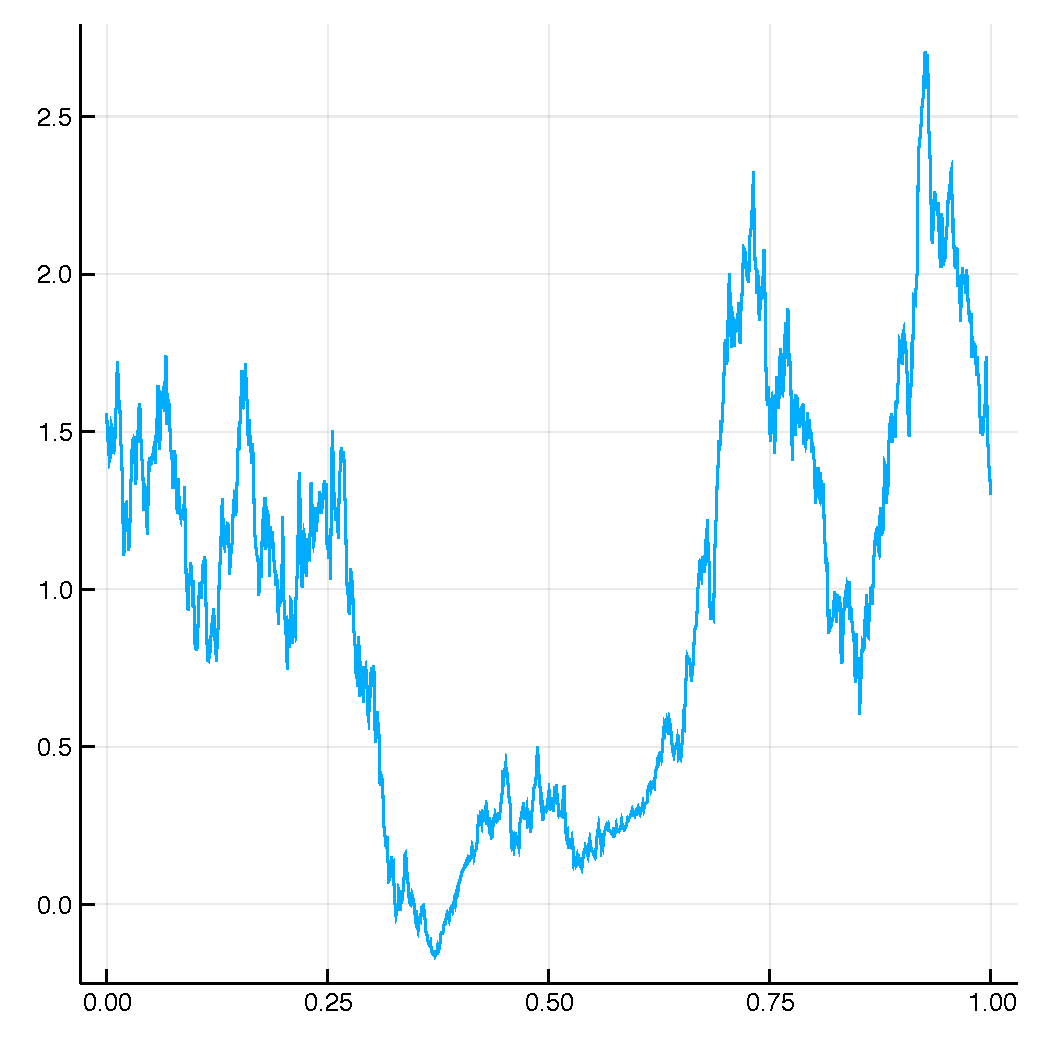
\includegraphics[width=\textwidth]{figures/scale2/dat-nss-p1000.pdf}
      \caption{Simulated random field}
    \end{subfigure}
    &
    \begin{subfigure}[t]{0.3\textwidth}
      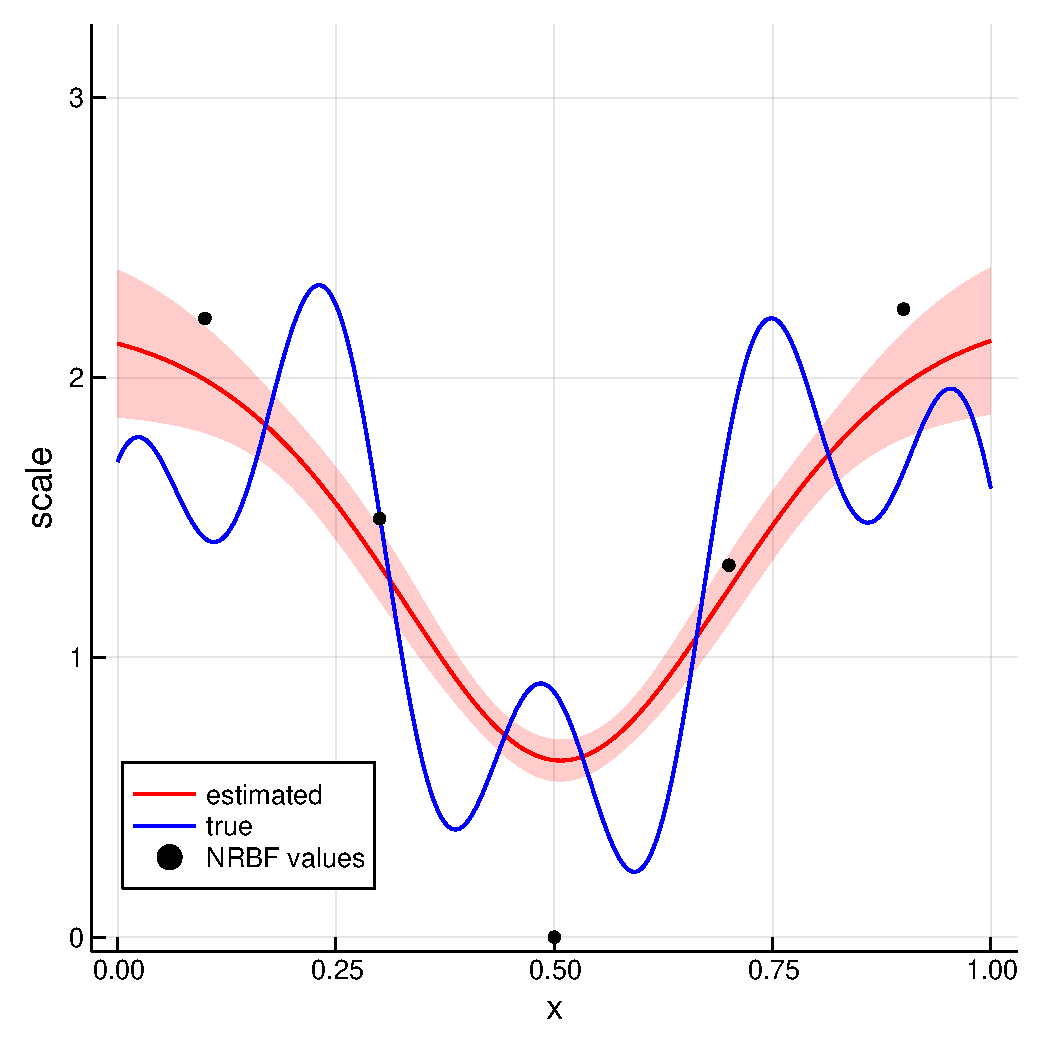
\includegraphics[width=\textwidth]{figures/scale2/est-p1000-a5-se1.pdf}
      \caption{Scale function \\ 5 basis functions}
    \end{subfigure}
    &
    \begin{subfigure}[t]{0.3\textwidth}
      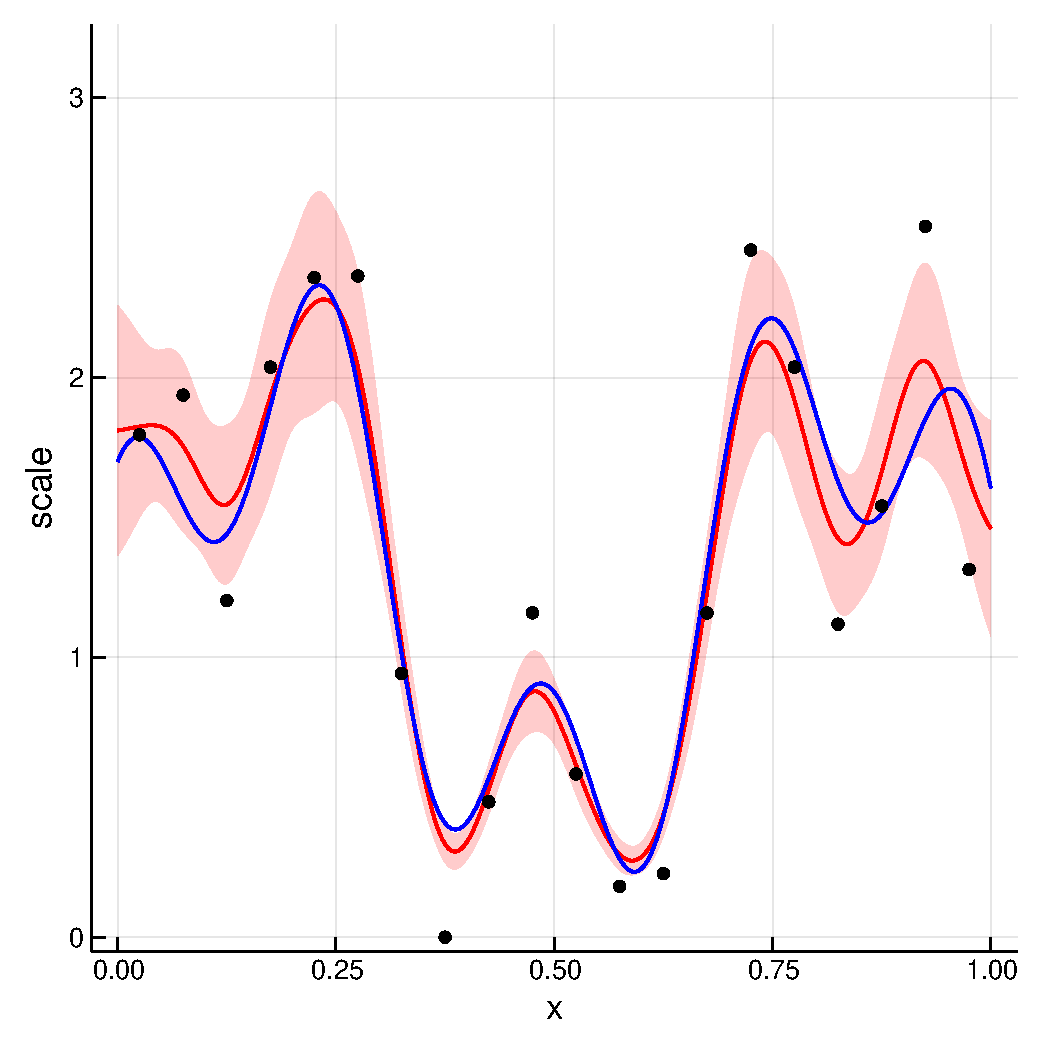
\includegraphics[width=\textwidth]{figures/scale2/est-p1000-a20-se1.pdf}
      \caption{Scale function \\ 20 basis functions}
    \end{subfigure}
  \end{tabular}
  \caption{Nonstationary scale parameter estimation for a 1D simulated random field. The isotropic Mat\'ern covariance with fixed $\Lambda=I$ and $\nu=1/2$ was used to generate 1,000 observations on a regular grid in $[0,1]$ with NRBF centers also on a regular grid. MLE computed using BFGS.}
  \label{fig:1d}
\end{figure}

\begin{figure}[H]
  \centering
  \begin{tabular}{cc}
    \begin{subfigure}[t]{0.3\textwidth}
      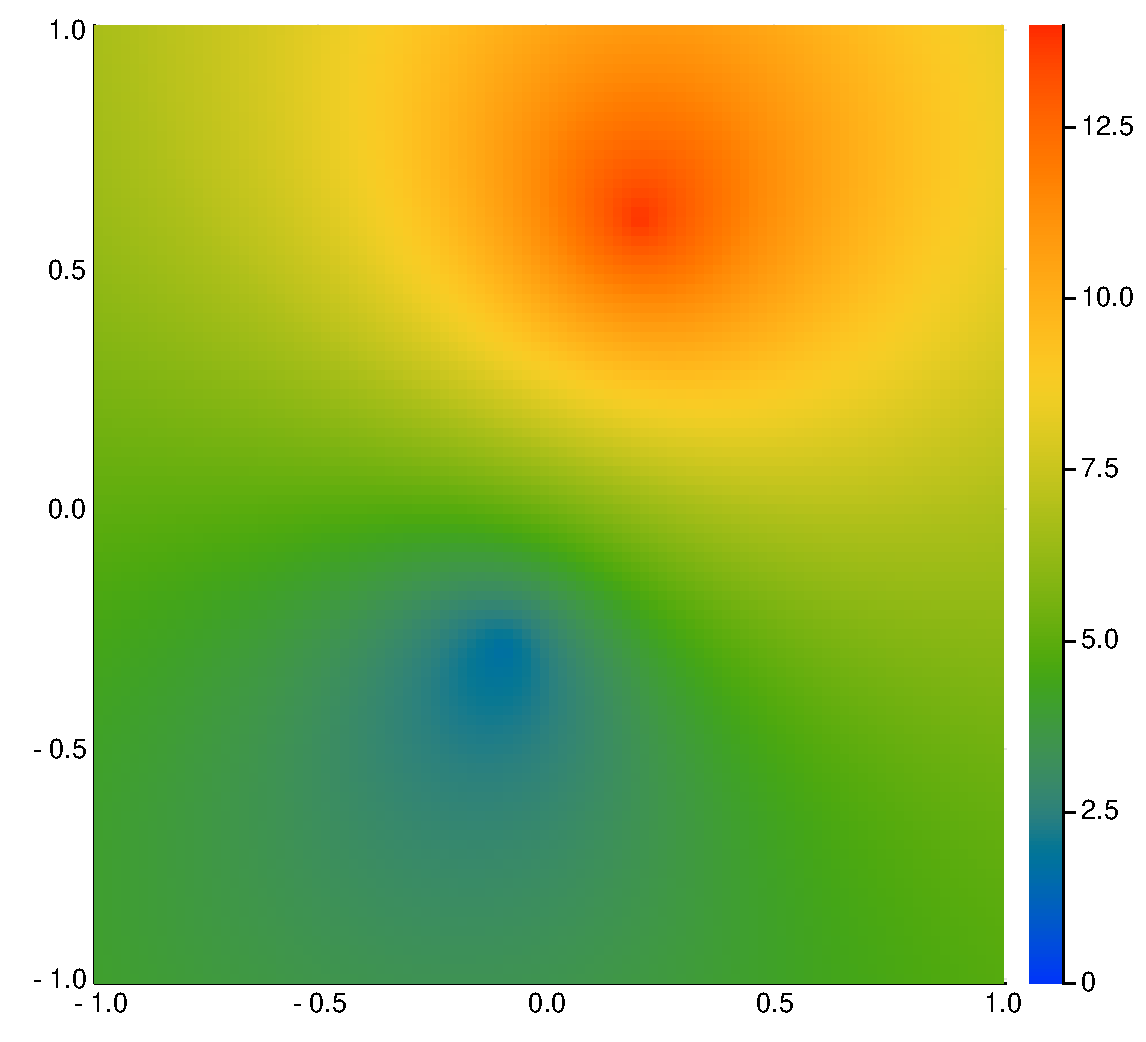
\includegraphics[width=\textwidth]{figures/isotropic/tru-nsr-p10000.pdf}
      \caption{True range function}
    \end{subfigure}
    & \begin{subfigure}[t]{0.3\textwidth}
      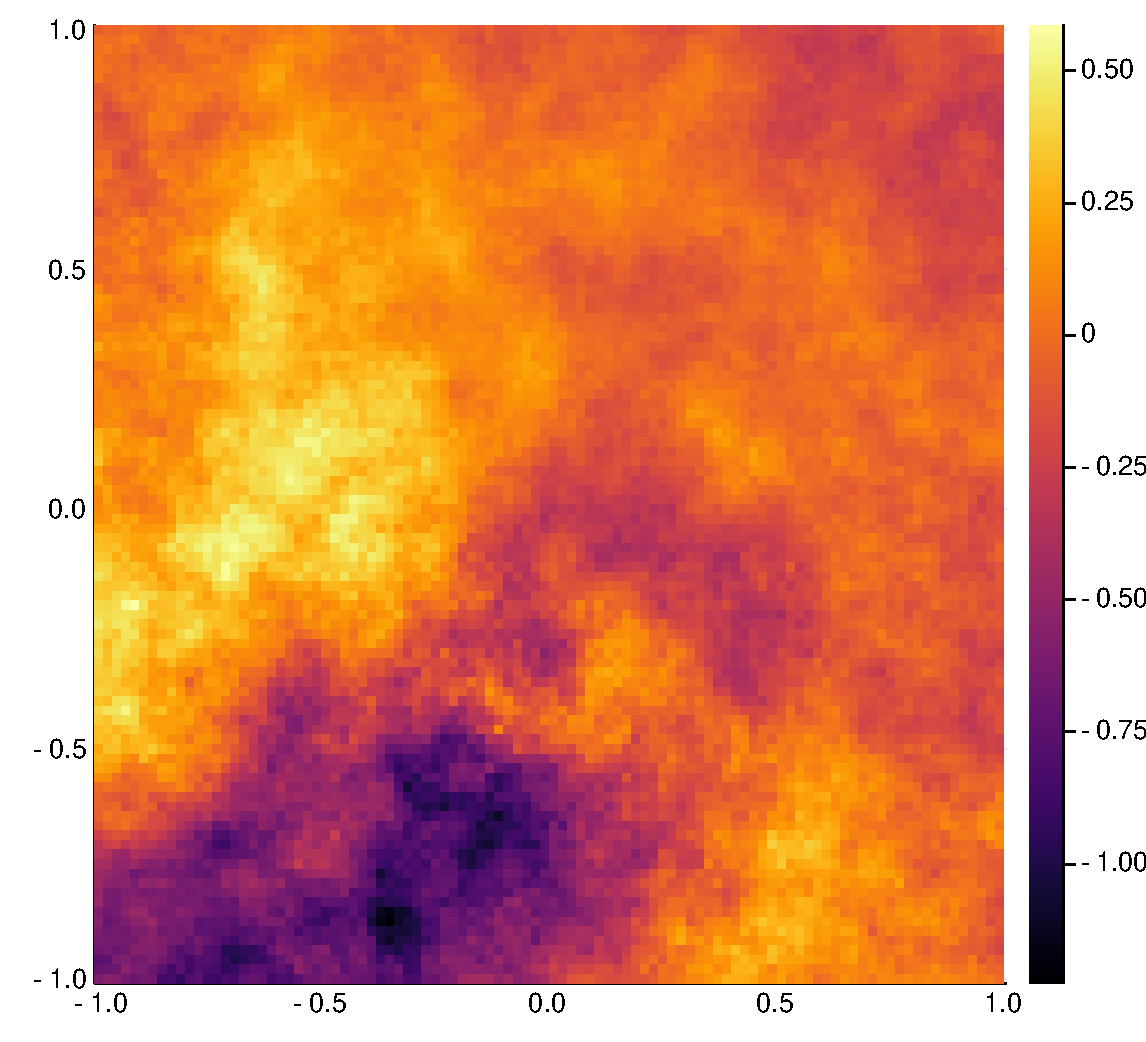
\includegraphics[width=\textwidth]{figures/isotropic/dat-nsr-p10000.pdf}
      \caption{Simulated random field}
    \end{subfigure} \\[6ex]
    \begin{subfigure}[t]{0.3\textwidth}
      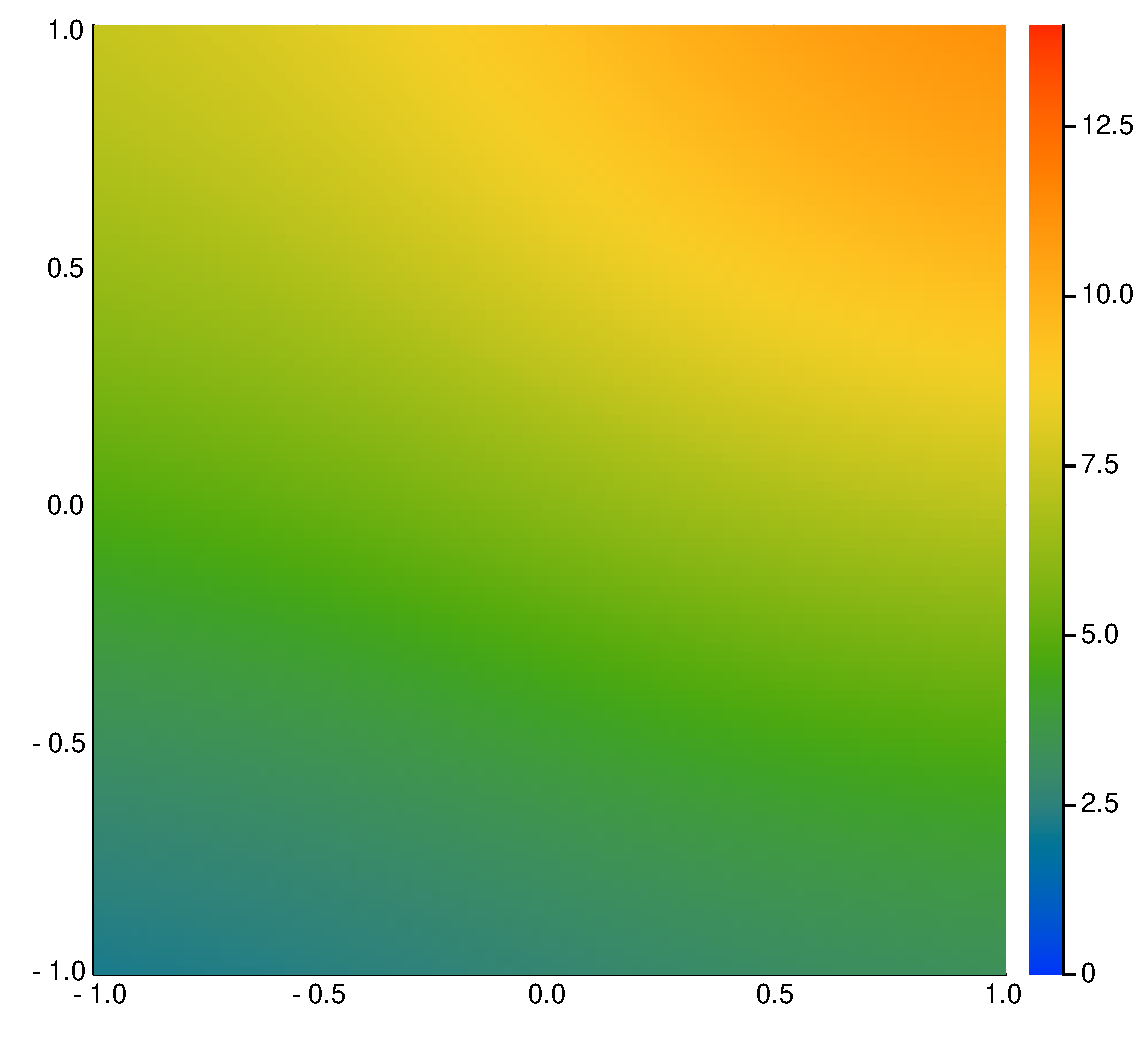
\includegraphics[width=\textwidth]{figures/isotropic/est-nsr-p10000-a4.pdf}
      \caption{Estimated range function \\ 4 basis functions}
    \end{subfigure}
    & \begin{subfigure}[t]{0.3\textwidth}
      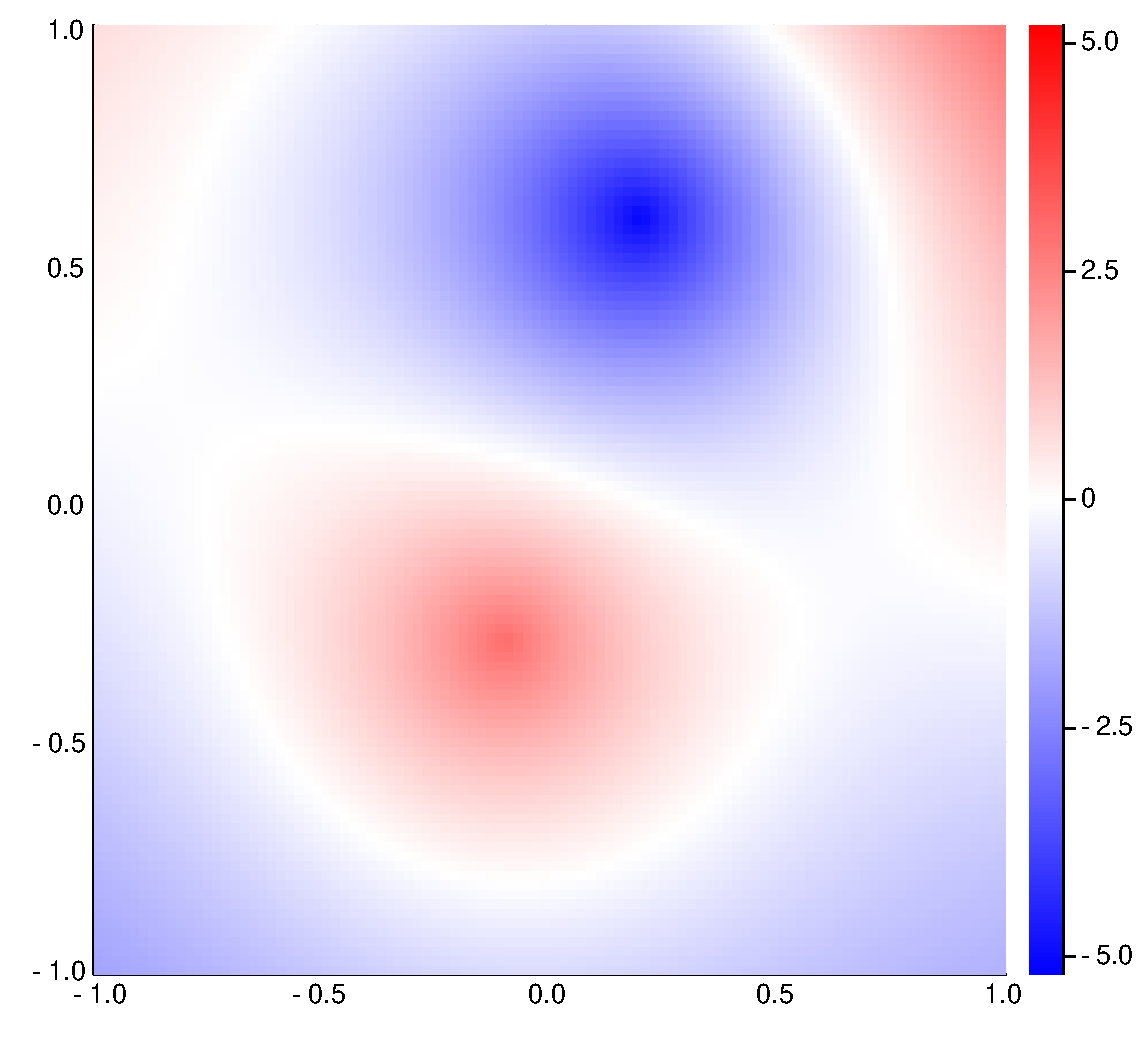
\includegraphics[width=\textwidth]{figures/isotropic/err-nsr-p10000-a4.pdf}
      \caption{Error \\ 4 basis functions}
    \end{subfigure} \\[6ex]
    \begin{subfigure}[t]{0.3\textwidth}
      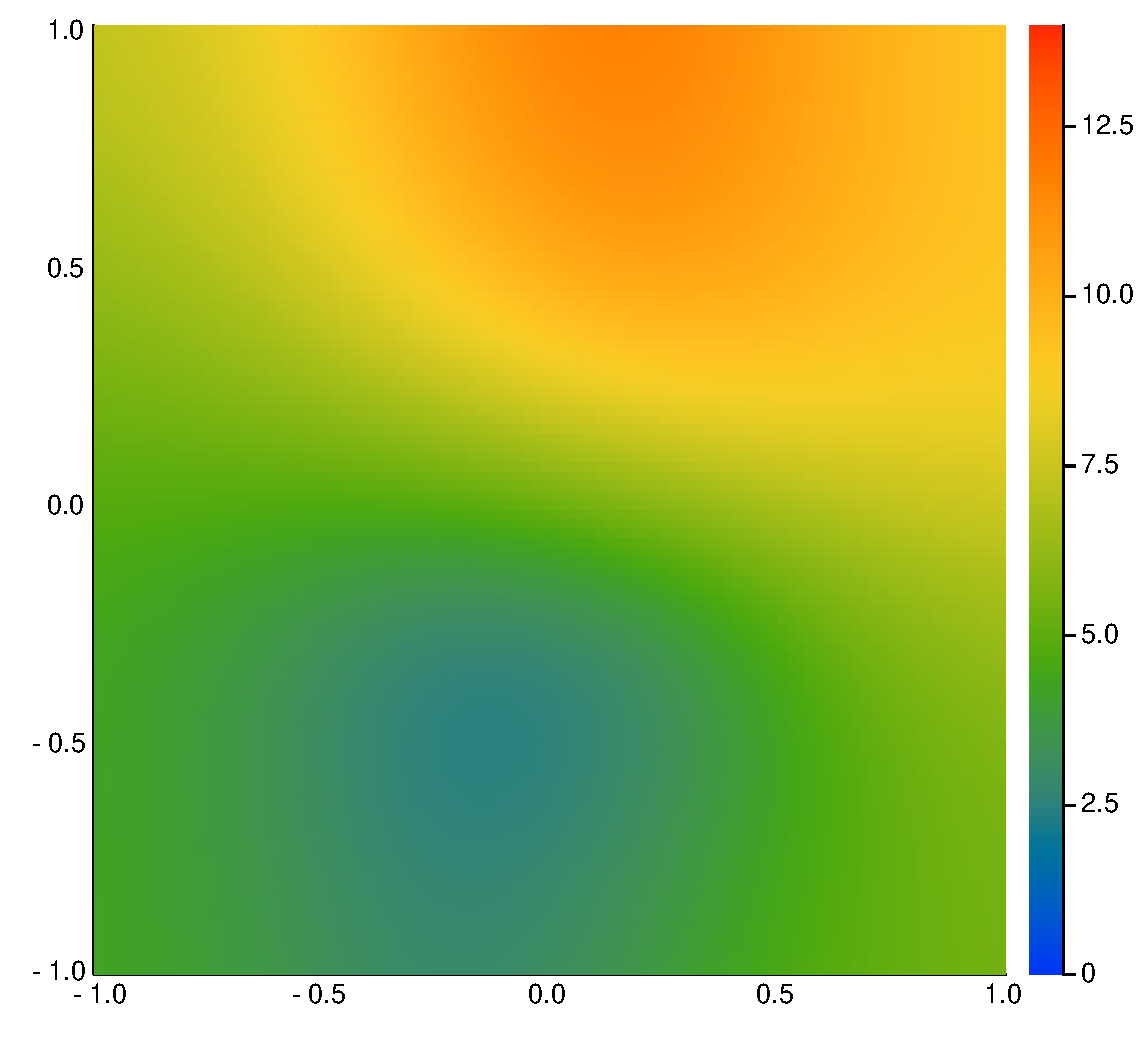
\includegraphics[width=\textwidth]{figures/isotropic/est-nsr-p10000-a16.pdf}
      \caption{Estimated range function \\ 16 basis functions}
    \end{subfigure}
    & \begin{subfigure}[t]{0.3\textwidth}
      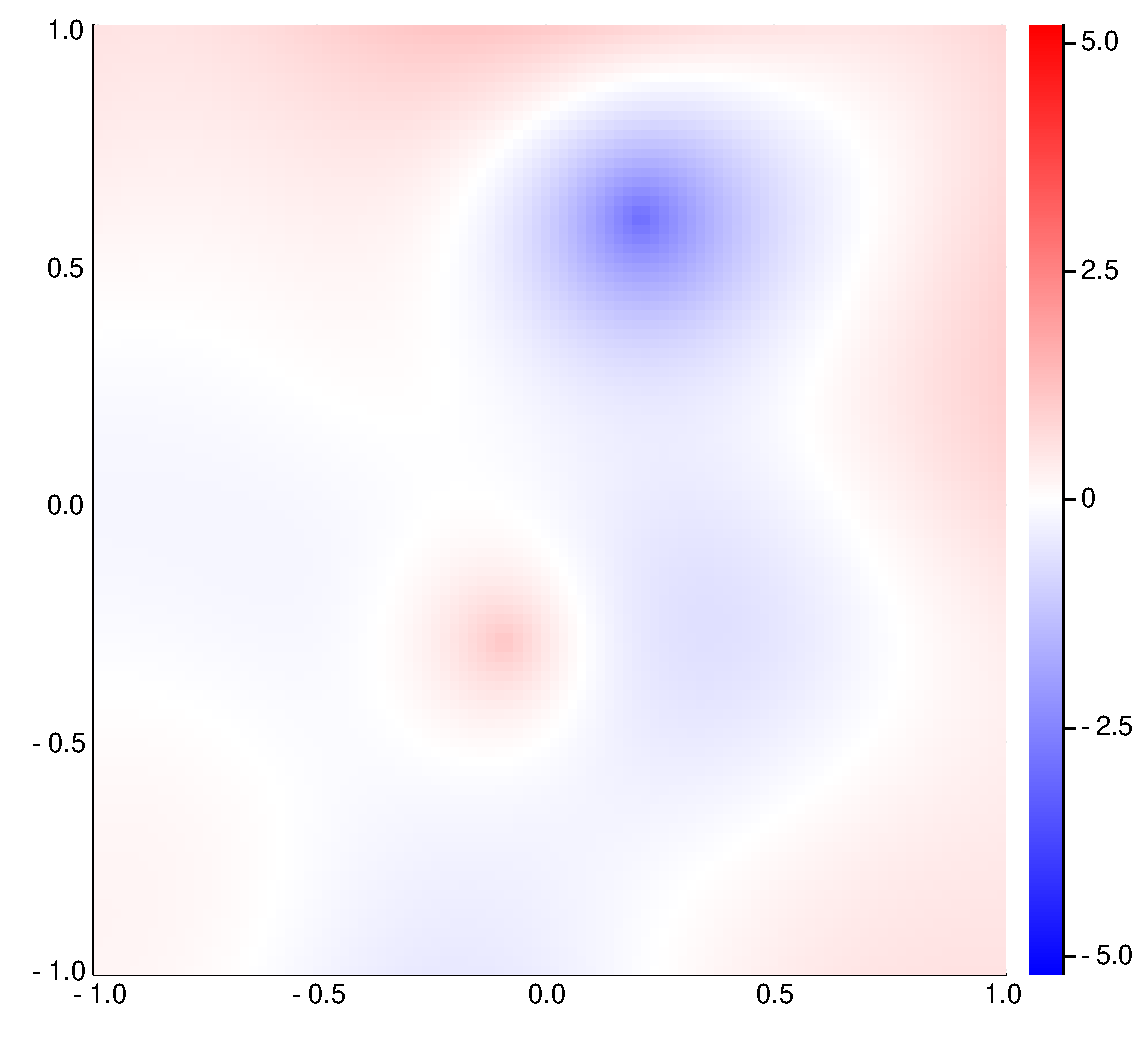
\includegraphics[width=\textwidth]{figures/isotropic/err-nsr-p10000-a16.pdf}
      \caption{Error \\ 16 basis functions}
    \end{subfigure}
    }
  \end{tabular}
  \caption{Nonstationary range parameter estimation for a 2D simulated random field. The isotropic Mat\'ern covariance with fixed $\sigma^2=1$ and $\nu=1/2$ was used to generate 10,000 observations on a regular grid in $[-1,1]^2$ with NRBF centers also on a regular grid. MLE computed using BFGS.}
  \label{fig:2d}
\end{figure}

\section{Conclusions and future directions} \label{sec:conclusions}

\bibliography{refs}{}
\bibliographystyle{plain}

\end{document}
